\section{AIT and Kolmogorov complexity}
\begin{frame}[label=intro3]{Kolmogorov complexity}

 We can think of agents as physical systems, and in turn,  of physical systems as dynamical systems implementing functions.   This allows us to analyze agents from the standpoint of computation theory.
 \begin{alertblock}{Warning: Computation is a mathematical concept}
The use of computational framework  in KT should not be construed to mean that the brain is literally a physical von Neumann computer (such as a laptop).
\end{alertblock}\vfill 
 
A computational perspective  leads us directly into algorithmic information theory (AIT) and its central concept: 


\begin{definition}[Kolmogorov complexity  of a dataset]
The length of the shortest program capable of generating  the dataset \citep{Kolomgorov1965,Cover:2006aa}.  
\end{definition} \vfill


\end{frame}

\begin{frame}[label=intro3]{Mutual algorithmic information ($\mathcal M$}

The {\em mutual algorithmic information  $\mathcal M(x,y)$ between two strings $x$ and $y$,   }
$$
\mathcal M(x \!:\!y) = \Ko(y)- \Ko(y|x),
$$
where $\Ko(y|x)$ is the complexity of the string $y$ if the computer has access to $x$ \citep{Li:1997aa, Grunwald:2004aa}.  
\end{frame}


\begin{frame}[label=ladila]{Model}
 With AIT as a basis, we can now define model and compressive/optimal model. \vfill 
 
 \begin{definition}[Model I]
 A  model  of a dataset is any program that generates the dataset. 
 \end{definition}
 Programs/models may differ in two ways: they may implement different functions, or they may implement the same function in different ways. Both aspects matter here:  we focus on programs that implement the right functions in the shortest possible way. \vfill 
 
\begin{definition}[K-model]
The optimal model or K-model of a dataset is the shortest program that generates (or, equivalently, compresses) the dataset.
\end{definition}
\end{frame}



\begin{frame}[label=ladila]{Model II}
An optimal model needs to capture and exploit all the structure in the dataset. In some sense, the {\em structure of the model can be described by the group of symmetries of the dataset}  \citep{Ruffini:2016ad}. 
 \begin{center}%\includegraphics[height=1.2cm]{COPL}%
  %\hspace{2cm}
  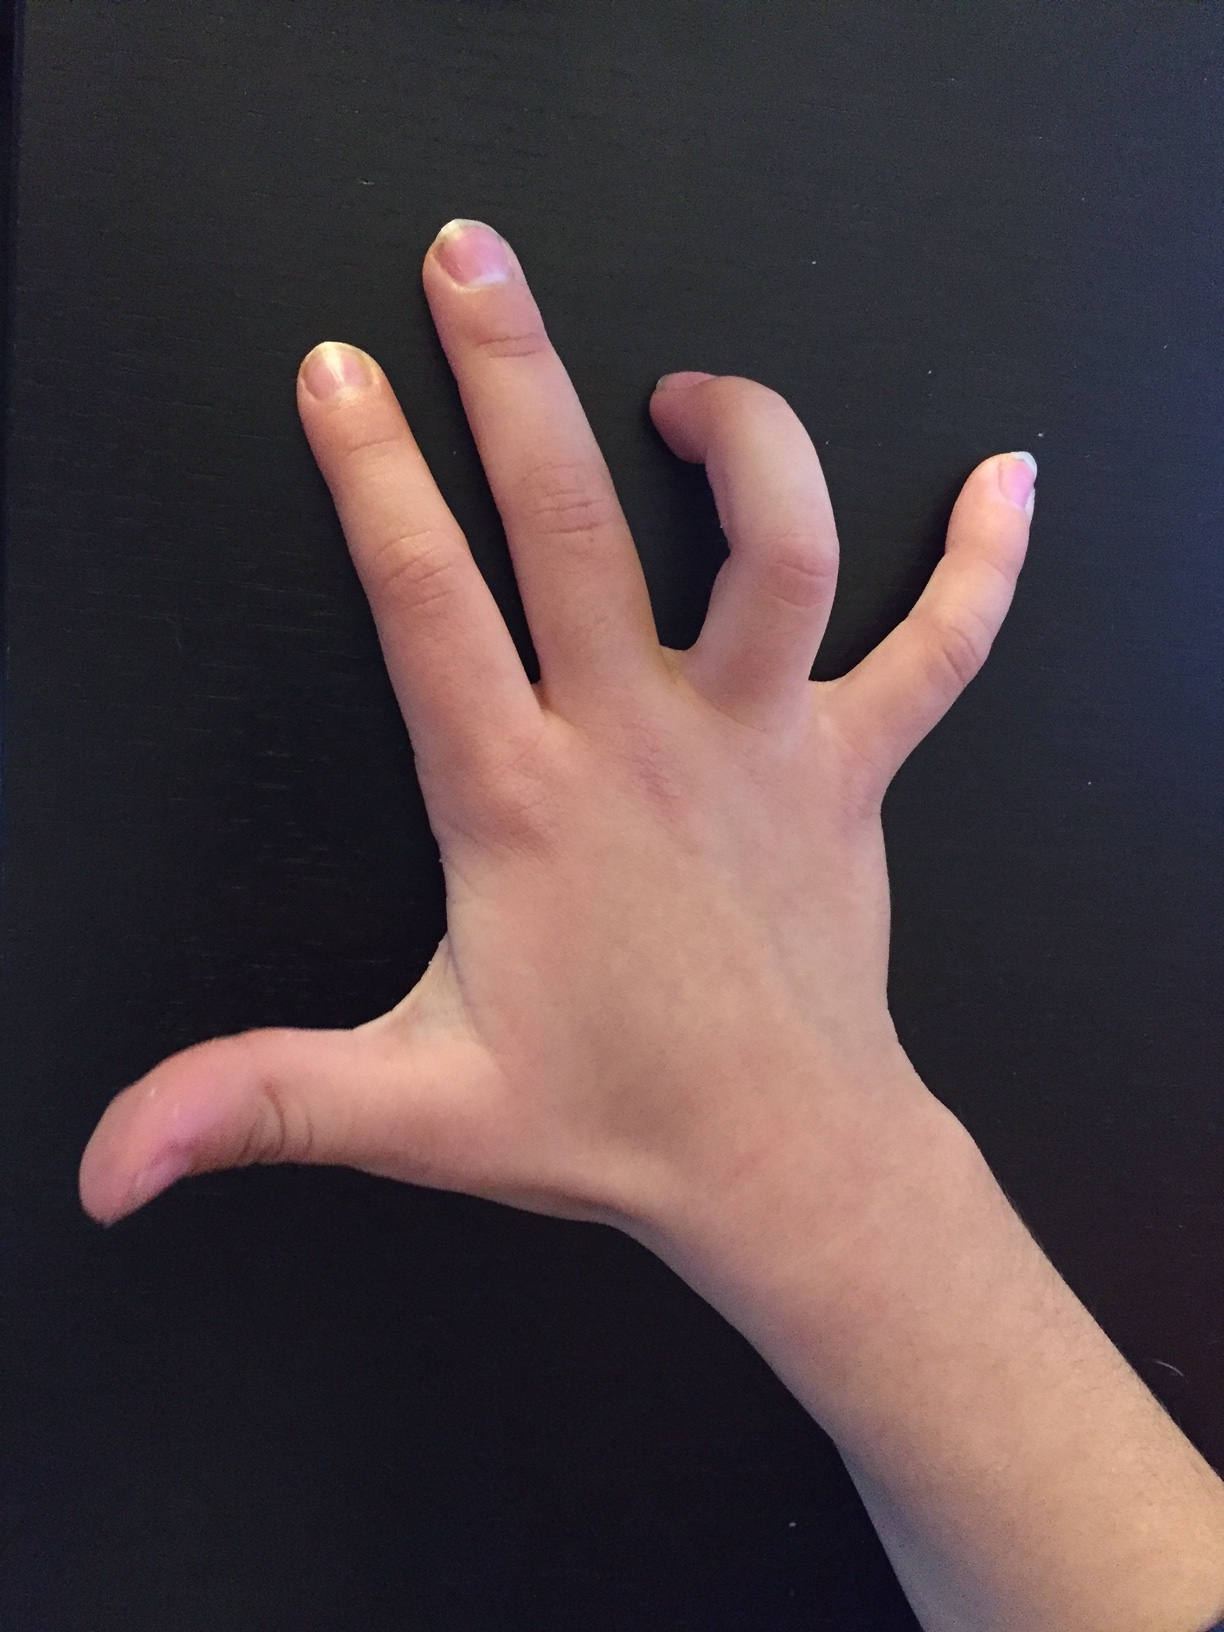
\includegraphics[height=4cm]{img/hand.jpeg}
  \end{center}
  
Suppose we are given a stack of images of a hand, e.g., from the frames of a movie of a moving hand  using a generating function,
$y = f(\theta)$, where $y$ is the image in a frame and $\theta$ a parametrization of the hand image and view.
\end{frame}

\begin{frame}[label=ladila]{Model III}
 \begin{center}%\includegraphics[height=1.2cm]{COPL}%
  %\hspace{2cm}
  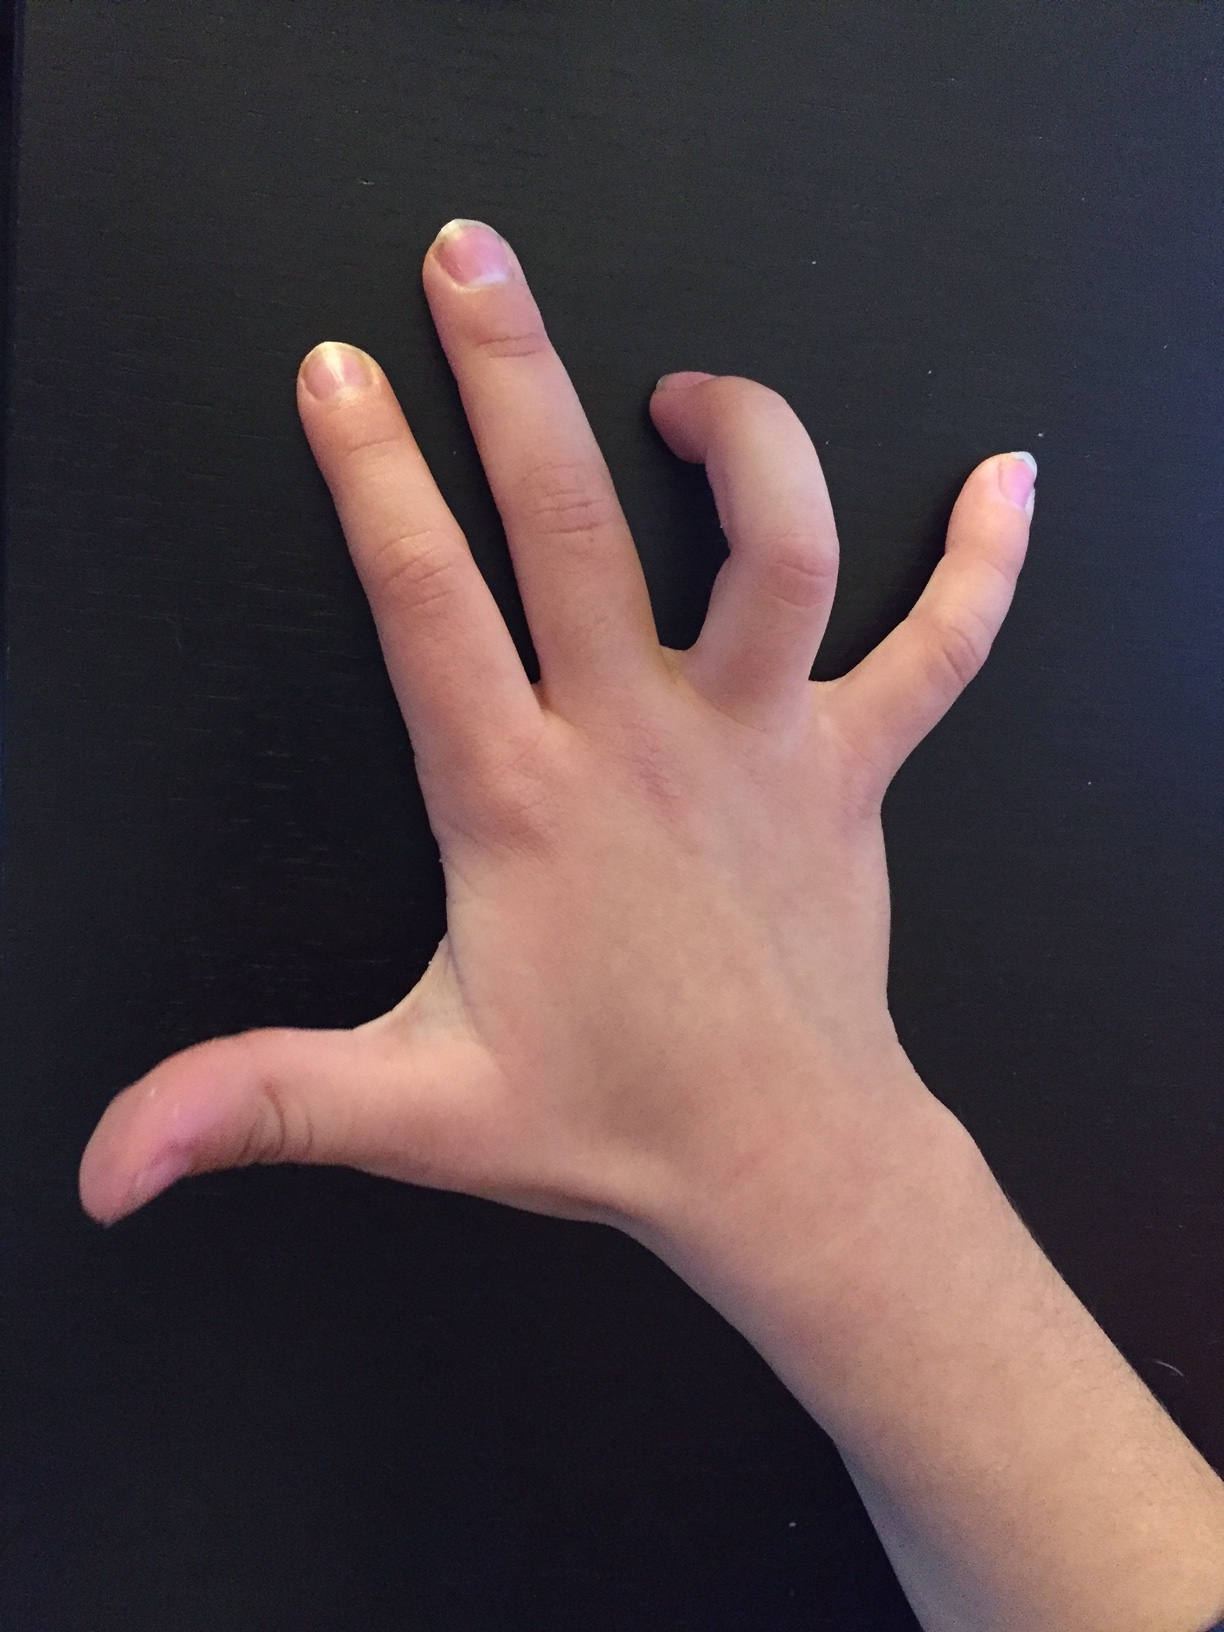
\includegraphics[height=4cm]{img/hand.jpeg}
  \end{center}
  The structure of the dataset is encapsulated by the function $f$, or the minimal program that encodes it and which is the {\em invariant} object.  The symmetries of the dataset are parametrized by $\theta$, and they are symmetries in the sense that if $\theta\rightarrow \theta'$ and $y\rightarrow y'$, then the equation $y'=f(\theta')$ holds true.
\end{frame}